\section{RESULTADOS}
Nesta se��o ser�o discutidos os resultados obtidos pelos diversos experimentos.
\subsection{PAM retangular}

Para o circuito da Figura \ref{f1}, temos os gr�ficos apresentados pelos oscilosc�pios na Figura \ref{fig_Osci1}.

\begin{figure}[H]
	\centering
	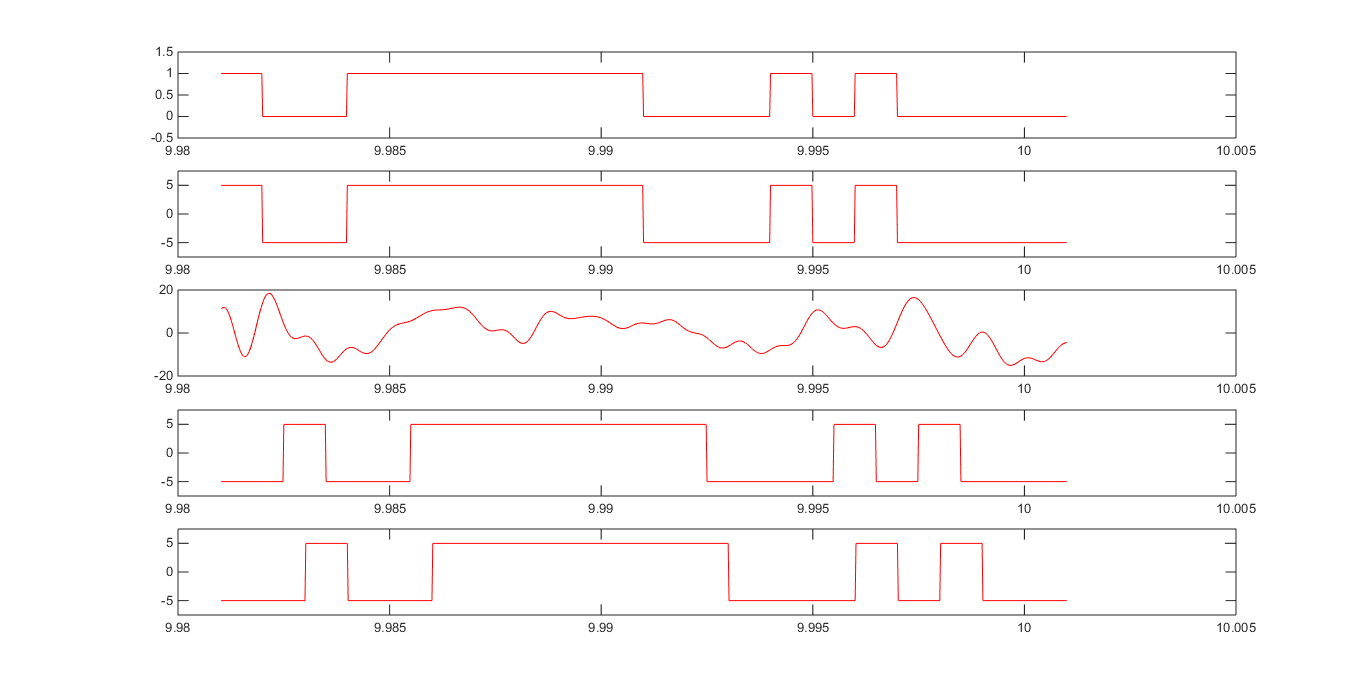
\includegraphics[scale=0.5]{Imagens/Ex2/23}
	\caption{Diversos sinais desde a modula��o � demodula��o.}
	\label{fig_Osci1}
\end{figure}

Por�m pelo fato de ter muitos gr�ficos na mesma imagem, foi optado pela plotagem de \textit{Tx} e \textit{Rx},pela Figura \ref{fig:atraso}, fica evidente o atraso de 3 bits para o dado circuito.

\begin{figure}[H]
	\centering
	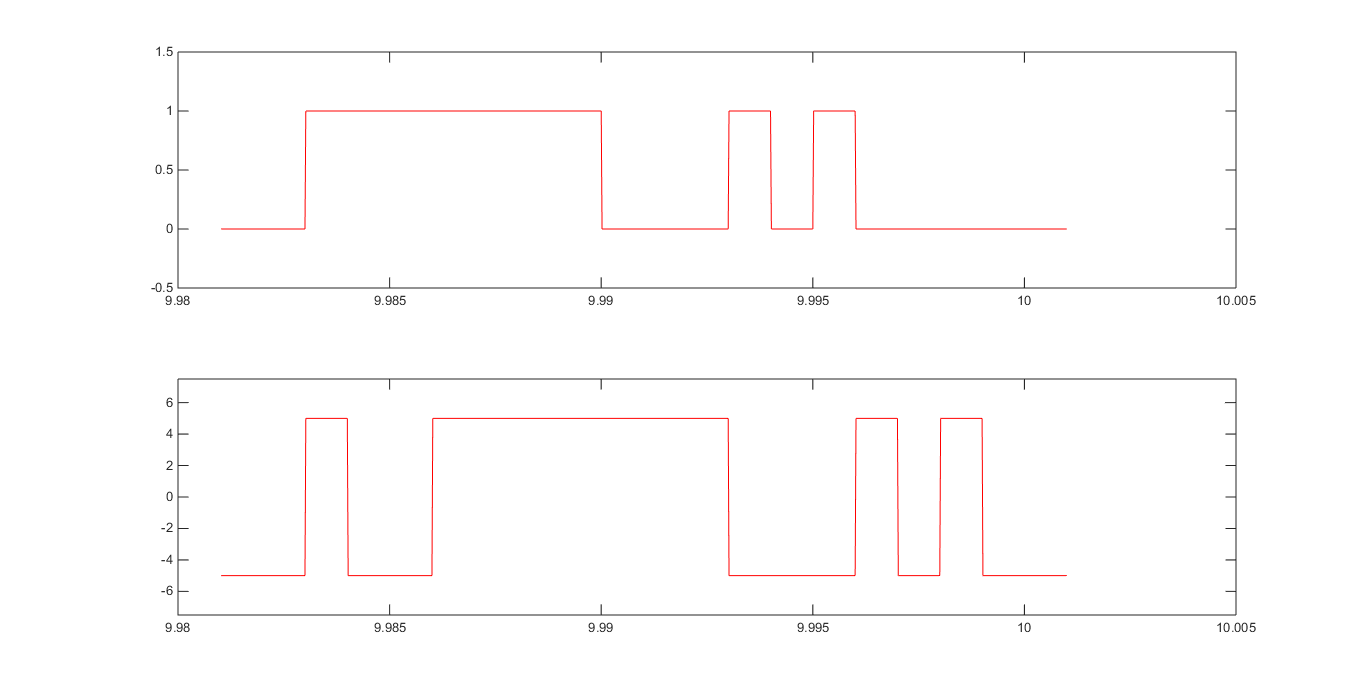
\includegraphics[scale=0.5]{Imagens/Ex2/atraso}
	\caption{Atraso entre Tx e Rx.}
	\label{fig:atraso}
\end{figure}

Com a simula��o devidamente configurada e variando $\sigma^2$ � poss�vel ent�o preencher a Tabela \ref{tab:ber1}.

\begin{center}
	\begin{table}[H]
		\caption{Taxa de erro de bit.}
        \label{tab:ber1}
		\centering\begin{tabular}{c|c|c}
			SNR[dB] & AWGN $\sigma^2$ & BER \\ \hline
			0,97   & 20 & 0,0000 \\
			-3,01  & 50 & 0,0001 \\
			-6,02  & 100 & 0,0051 \\
			-7,78  & 150 & 0,019  \\
			-9,03  & 200 & 0,036  \\
			-10,00 & 250 & 0,052  \\
			-10,33 & 270 & 0,059  \\
			-10,79 & 300 & 0,066  \\
			-13,01 & 500 & 0,11  \\ \hline
		\end{tabular}
	\end{table}
\end{center}

Assim a Figura \ref{fig:BER1}, apresenta o gr�fico da \textit{SNR} por \textit{BER}.

\begin{figure}[H]
	\centering
	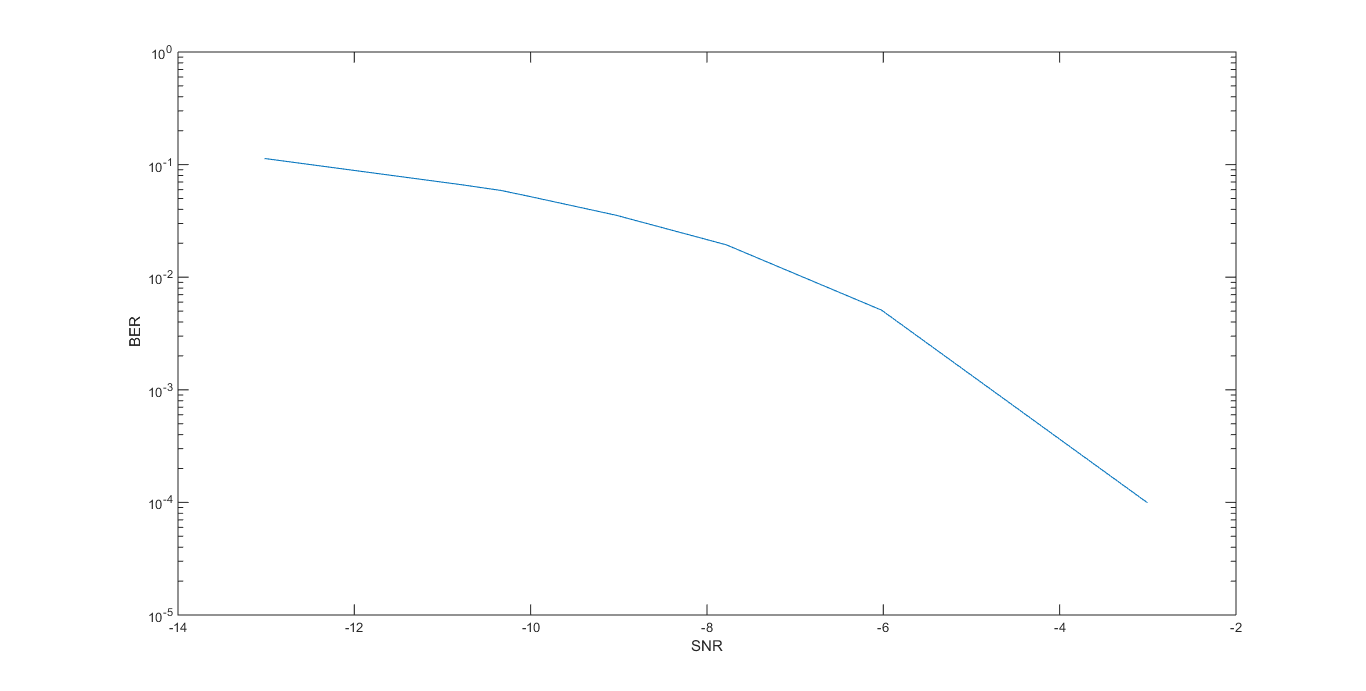
\includegraphics[scale=0.5]{Imagens/Ex2/SNRxBER}
	\caption{Taxa de erro de bit em fun��o da rela��o sinal ru�do.}
	\label{fig:BER1}
\end{figure}

\subsection{PAM sinc}

Com o PAM modulado com sinc da Figura \ref{f2}, foi obtido o gr�fico presente na Figura \ref{fig:sincCent} e \ref{fig:sincMili}.

\begin{figure}[H]
	\centering
	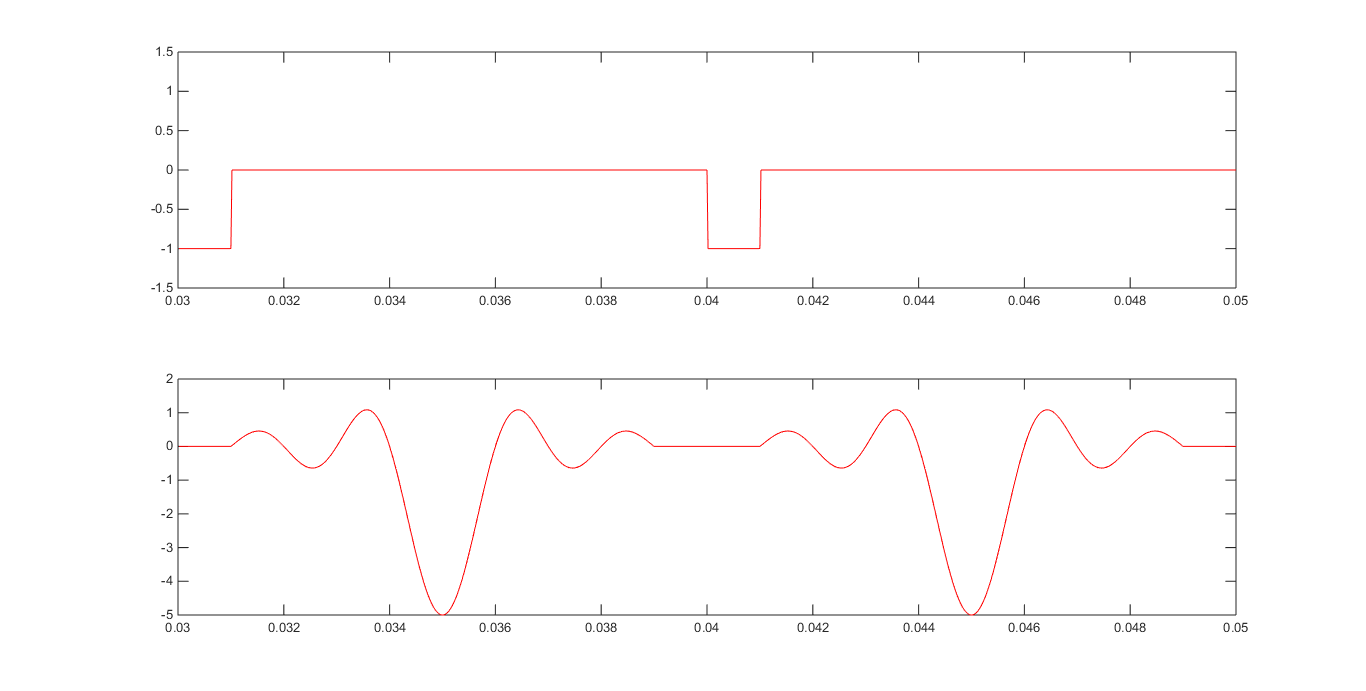
\includegraphics[scale=0.5]{Imagens/Ex3/cent}
	\caption{PAM sinc com taxa de $10^2$.}
	\label{fig:sincCent}
\end{figure}

\begin{figure}[H]
	\centering
	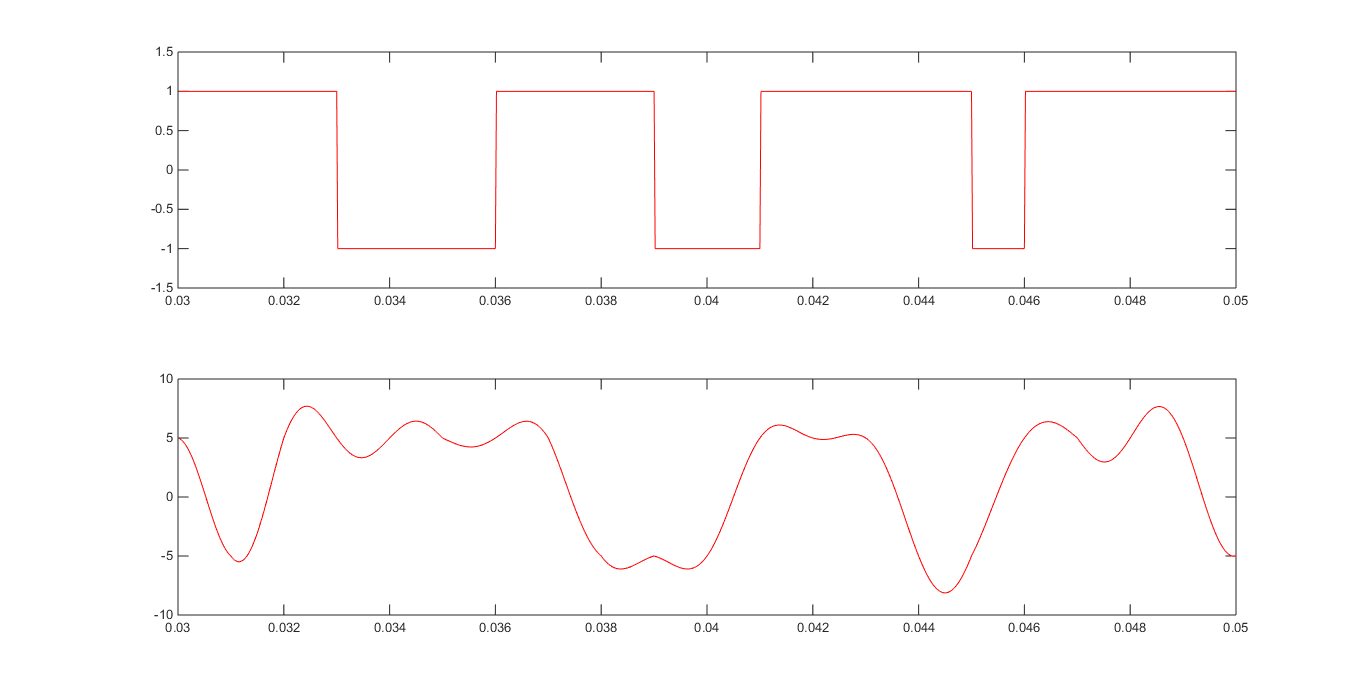
\includegraphics[scale=0.5]{Imagens/Ex3/mili}
	\caption{PAM sinc com taxa de $10^3$.}
	\label{fig:sincMili}
\end{figure}

Para validar a teoria ent�o � colocado um elemento para analisar a \textit{PSD}, densidade espectral de pot�ncia, apresentado na Figura \ref{fig:PSD}.

\begin{figure}[H]
	\centering
	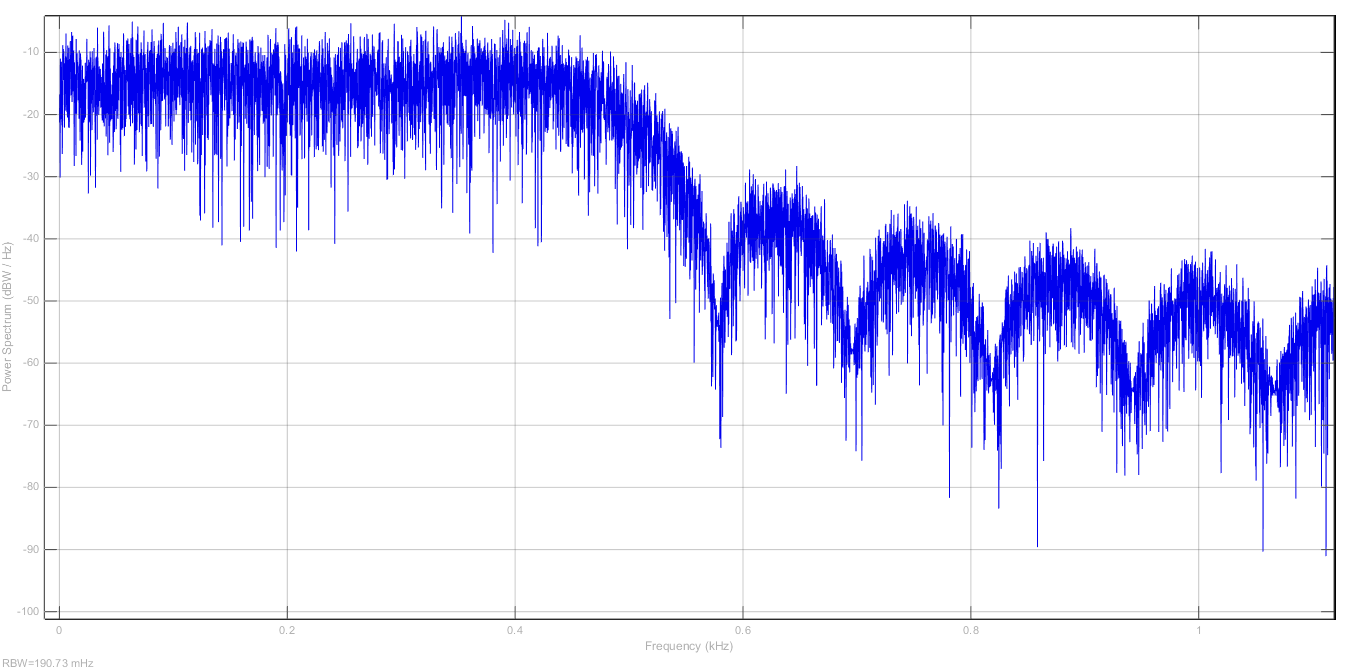
\includegraphics[scale=0.5]{Imagens/Ex4/PSDZOOM}
	\caption{PSD para PAM sinc.}
	\label{fig:PSD}
\end{figure}

Desta forma a frequ�ncia de joelho, � $f_c\approx0,5[kHz]$ o que comprova a teoria pois a banda de um sinal amostrado por uma sinc � metade de um amostrado por uma retangular.

\subsection{PAM sinc por um canal AWGN}

Para o circuito da Figura \ref{f3}, � analisado o atraso a partir da Figura \ref{fig:Rxdemo}.

\begin{figure}[H]
	\centering
	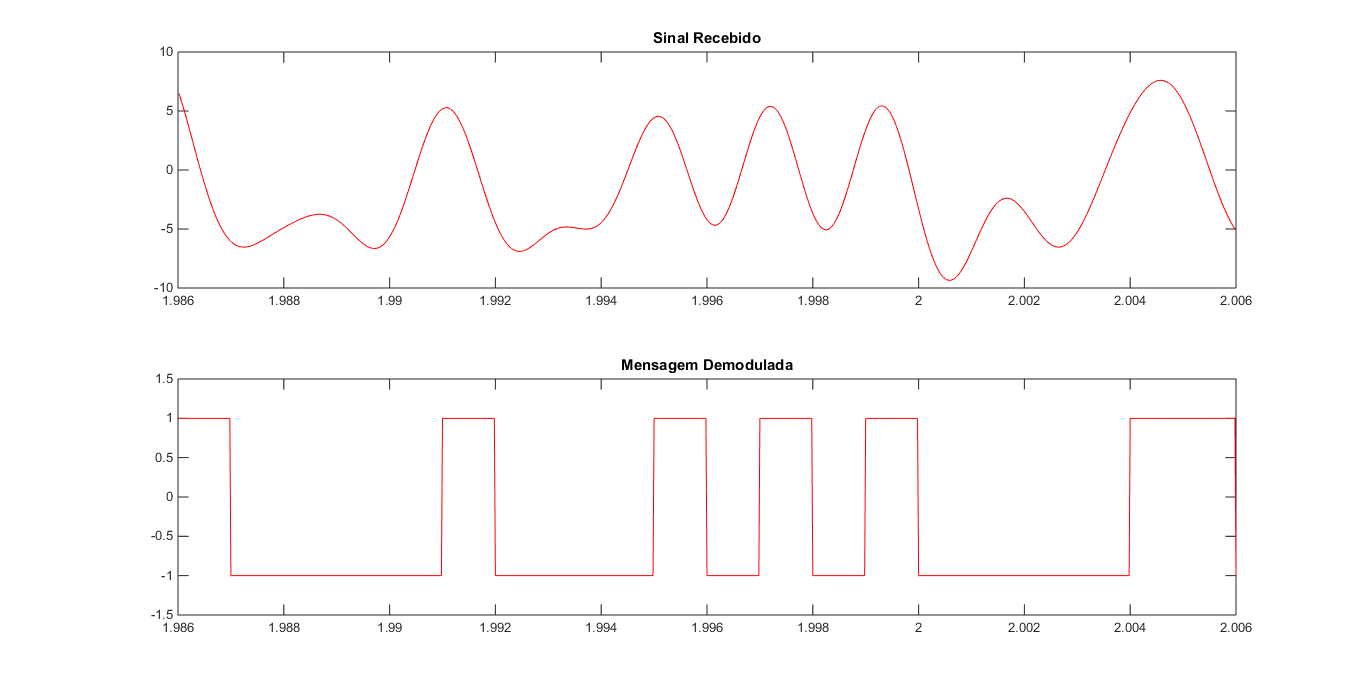
\includegraphics[scale=0.5]{Imagens/Ex5/RxDemo}
	\caption{PAM sinc por um canal AWGN.}
	\label{fig:Rxdemo}
\end{figure}

Assim o atraso de 6 bits fica evidente pela Figura \ref{fig:atraso2}.

\begin{figure}[H]
	\centering
	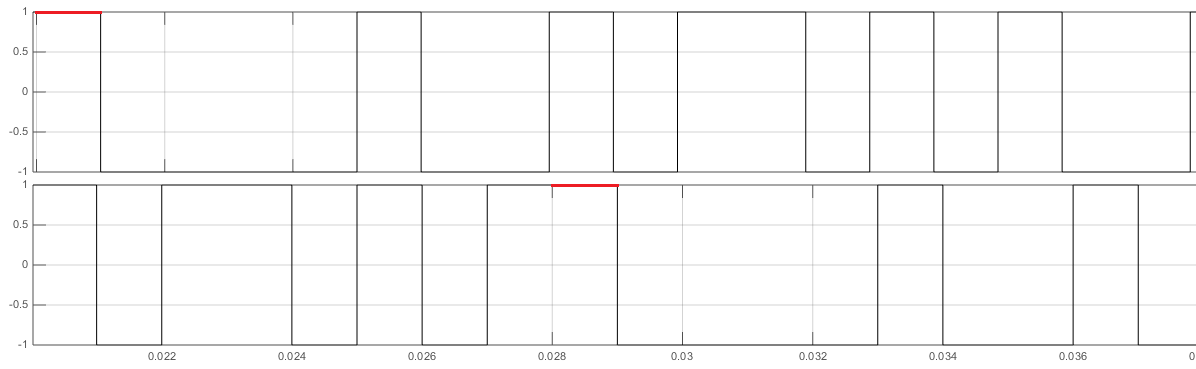
\includegraphics[scale=0.5]{Imagens/Ex5/atraso2}
	\caption{Atraso de 6 bits.}
	\label{fig:atraso2}
\end{figure}

Por fim, para fazer um comparativo e tabelado os valores para diversos $\sigma^2$, de maneira similar a se��o 5.1, obtendo os valores presente na Tabela \ref{tab:ber2}.

\begin{center}
	\begin{table}[H]
		\caption{Taxa de erro de bit.}
		\centering\begin{tabular}{c|c|c}
			SNR[dB] & AWGN $\sigma^2$ & BER \\ \hline
0,85   & 20  & 0      \\
-3,13  & 50  & 0,0004 \\
-6,14  & 100 & 0,004  \\
-7,90  & 150 & 0,011  \\
-9,15  & 200 & 0,023  \\
-10,12 & 250 & 0,030  \\
-10,46 & 270 & 0,037  \\
-10,92 & 300 & 0,046  \\
-13,13 & 500 & 0,091 \\ \hline
		\end{tabular}
		\label{tab:ber2}
	\end{table}
\end{center}

Por fim � realizado um gr�fico comparativo entre o circuito PAM \textit{retangular} e o \textit{sinc}, presente na Figura \ref{fig:BERcomp}.

\begin{figure}[H]
	\centering
	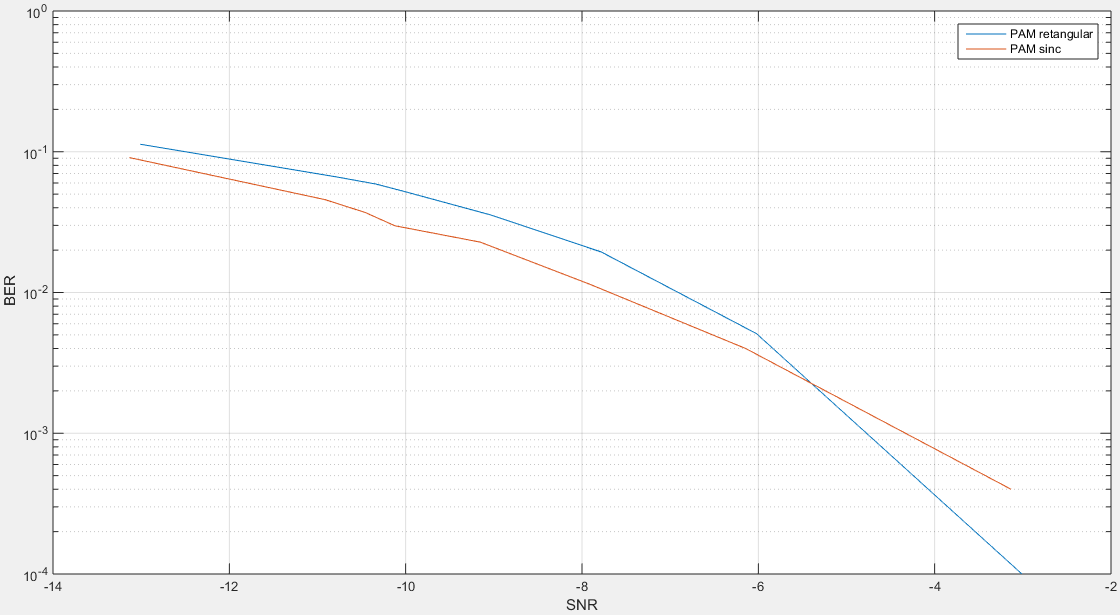
\includegraphics[scale=0.5]{Imagens/Ex5/BERcomp}
	\caption{Comparativo entre os dois tipos de modula��o.}
	\label{fig:BERcomp}
\end{figure}


\newpage
